%! TeX program = luatex
\documentclass[9pt]{beamer}

\usepackage{physics, amsmath, amsfonts,amssymb}
\usepackage{tikz}
\usetikzlibrary{arrows.meta, fit, positioning}

\usetheme{metropolis}
\title{When does a system admit an equilibrium probability distribution}
\author[Sabarno Saha]{Sabarno Saha \inst{1} }
\institute[IISERK]{\inst{1} Department of Physical Sciences IISERK}
\date{\today}
  \metroset{block=fill}
  \newcommand{\A}{\mathbb{A}}
  \newcommand{\X}{\mathbb{X}}
  \newcommand{\Y}{\mathbb{Y}}
  \newcommand{\Z}{\mathbb{Z}}
  \newcommand{\PP}{\bold{P}}

\begin{document}

\frame{\titlepage}

\begin{frame}
  \frametitle{Introduction}
  \begin{enumerate}
    \item Stochastic Description
      \begin{itemize}
        \item Stochastic Processes
        \item Markov Chains
        \item CTMC 
        \item Transition Rate Matrix
      \end{itemize}
    \item Steady State and Equilibrium Distribution
      \begin{itemize}
        \item Conditions
        \item Detailed Balance Condition
      \end{itemize}
    \item Perron Frobenius Theorem
      \begin{itemize}
        \item Irreducibility
        \item Strongly connected graphs
        \item Stationary State distribution
      \end{itemize}
  \end{enumerate}
\end{frame}

\begin{frame}
  \frametitle{Introduction(Contd.)}
  \begin{enumerate}\setcounter{enumi}{4}
    \item Graph/ Network Theory
      \begin{itemize}
        \item Graphs
        \item Trees
        \item Handshaking lemma
        \item An "obvious" theorem
      \end{itemize}
    \item Equilibrium Distribution
  \end{enumerate}

\end{frame}


\section{A Stochastic Description}
\begin{frame}
  \frametitle{Stochastic Process}
  \metroset{block=fill}
  \begin{block}{Stochastic Process}

    A stochastic process is a sequence of random variables where the indexing of the variables
    often carries the notion of time. 

  \end{block}

  An example would be Brownian Motion, which is described by the Wiener process.
  % $$ P(x,t) = \frac{1}{\sqrt{2\pi t}} \exp(\left(-\frac{x^2}{2t}\right)$$
  \begin{displaymath}
      P(\hat{W}(t+\Delta t)=x | \hat{W}(t)=x') = \frac{1}{\sqrt{2 \pi \Delta t}}\exp(-\frac{(x-x')^2}{2 \Delta t})
    \end{displaymath}

\end{frame}
% \begin{frame}
%   \frametitle{Brownian Motion}
%   Here, we simulate the Brownian motion using the Wiener process(using Gillespie's algorithm).

% \end{frame}
\begin{frame}
  \frametitle{Markov Chains}
  Most of the physical processes that we study in classical statistical physics is modelled as
  Markov Chains. 
  \begin{block}{Markov Property}
    Let $ \{X_n\}$ be a stochastic process.
    The markov property is defined as
    $$\mathbb{P}(X_{n+1}|X_n,X_{n-1},...,X_0) = \mathbb{P}(X_{n+1}|X_n)$$
    Any stochastic process satisfying the Markov property is called a Markov Chain.
  \end{block}
  Essentially the future of the system is independent of the past given the present state.

\end{frame}

\begin{frame}
  \frametitle{Continuous Time Markov Chains(CTMC)}
  These are markov chains with the index as time $\{X(t)\}_t$. Let us define a state space as the 
  set of all values $S$ a random variable can assume. Then we use the notation 
  $$ P(X(t) = s) \equiv P(s;t)$$
  We can rewrite the markov property as 
  $$ P(s_n;t_n|s_{n-1};t_{n-1},s_{n-2};t_{n-2},...,s_0;t_0) = P(s_n;t_n|s_{n-1};t_{n-1})$$
  where $s,s_i \in S ~ \forall i$.

  Now using the theorem of total probability we can write the Chapman Kolmogorov equation as
  \begin{block}{Chapman Kolmogorov Equation}
  $$ P(s;t|s_0;t_0) = \sum_{s' \in S} P(s;t|s';t')P(s';t'|s_0;t_0)$$ where $t > t' > t_0$
  \end{block}
\end{frame}
\begin{frame}
  \frametitle{Continuous Time Markov Chains(CTMC)}
  We now choose a time interval $dt$ and rewrite the Chapman Kolmogorov equation, dropping the 
  explicit dependence on $x_0,t_0$
  $$ P(s;t+dt) = \sum_{s' \in S} P(s;t+dt|s';t)P(s';t)$$
  Since this is an infinitesimal time interval, we can write the above equation as
  $$ P(s;t+dt|s';t) = \delta_{ss'} +Q_{ss'}dt + o(dt)$$
  where $Q$ is the transition rate matrix. 
\end{frame}

\begin{frame}
  \frametitle{Transition Rate Matrix}
  The transition rate matrix should satisfy the following conditions 
  \begin{enumerate}
    \item $Q_{ss'} \geq 0$ for $s \neq s'$
    \item $Q_{ss} = -\sum_{s' \neq s} Q_{ss'}$
  \end{enumerate}
  The first condition ensures that the transition rate is non-negative and the second condition
  essentially ensures that the probability of transitioning from a state $s$ to any state is 1.
  
  Thus we can write 
  $$\mathbb{P}(t+dt) = \mathbb{I} + Qdt$$ where $\mathbb{I}$ is the identity matrix.

\end{frame}

\begin{frame}
  \frametitle{Transition Rate Matrix}
  We define $k_{xx'}$ as the jump rate from state $x'$ to $x$.
  We thus define the elements of the transition rate matrix as
  $$ p(x;t+dt|x';t' ) = Q_{xx'} = k_{xx'} \quad \quad x \neq x'$$
  And the diagonal elements are thus given as 
  $$Q_{xx} = -\sum_{x' \neq x} k_{xx'}$$

  We also assume that the elements $k_{xx'}$ do not change with time.

  The change in probability of being in state $x$ at time $t$ is the \textbf{inflow} of probability from all other states
  which is $ k_{xx'}p(x';t)$ minus the \textbf{outflow} of probability  $k_{x'x}p(x;t)$.
  We can now write the master equation as
  $$\dv{p(x;t)}{t} = \sum_{x' \in S} k_{xx'}p(x';t) - k_{x'x}p(x;t)$$
  This becomes clearer when we define the probability current.
\end{frame}

\begin{frame}
    \frametitle{Master Equations}
    These equations describe the time evolution of the system that are modelled as being in the
    a probabilistic combination of a set of states at any given time. These are phenomenologically modelled 
    first order differential equations. 

    These are used in a variety of fields in physics, and other related fields. These are used for 
    studying birth and death processes, non-equilibrium statistical mechanics, chemical reactions, and a whole lot more. \\ 

    The most common one that we see is the one used here is of the form 
    $$ \frac{d \bold{p}}{ dt} = \A \bold{p} $$
    where $\A$ is the matrix of connections and $\bold{p}$ is the probability distribution column vector.
\end{frame}
\begin{frame}
  \frametitle{Probability Current}
  \begin{block}{Probability Current}
    The probability current is defined as the flow of probability from state $x'$ to state $x$.
    We define the probability current as
    $$J_{xx'} = k_{xx'}p(x';t) - k_{x'x}p(x;t)$$
  \end{block}
    The master equation can now be written as
    $$\dv{p(x;t)}{t} = \sum_{x' \in S} J_{xx'}$$

    A bit of physics coming up ahead $:)$
    
    \begin{block}{Microscopic Reversibility}
      If for any allowed jump $x \rightarrow x'$(i.e. $k_{xx'} > 0$), the reverse jump $x' \rightarrow x$ $(k_{x'x}>0)$ is also allowed, then the system is said to be microscopically reversible.
  
    \end{block}

\end{frame}
\begin{frame}
  \frametitle{Jump Networks}
  These systems are quite often represented as jump networks, where the nodes of the graph 
  represent the states $x$ and the arrows(edges) $ x' \rightarrow x$ represent the allowed jumps  
  i.e. the jumps with non-zero transition rates($k_{xx'}>0$).

  \begin{block}{Some Physics}
    The \textbf{jump networks} dealt with in physics are \textbf{strongly connected}. 
    That is, given any two states $x$ and $x'$, there is a non-zero probability 
    of transitioning from $x$ to $x'$ in a finite number of steps.
\end{block}
This property has some physical justification. Coupled together with microscopic reversibility, 
this property ensures that the graphs aren't disconnected. Disconnected graphs often lead to systems 
with non-interacting components, which can be studied independently reducing to the strongly connected graph.
\\
\end{frame}
\begin{frame}
  \frametitle{Jump Networks}

  \emph{Strongly connected graphs also posses a property called Irreducibility. Irreducibility is a necessary condition for the Perron Frobenius theorem to hold.}
\end{frame}

\begin{frame}
  \frametitle{Jump Networks}
    Here are is an example of a jump network : 
  \begin{figure}
    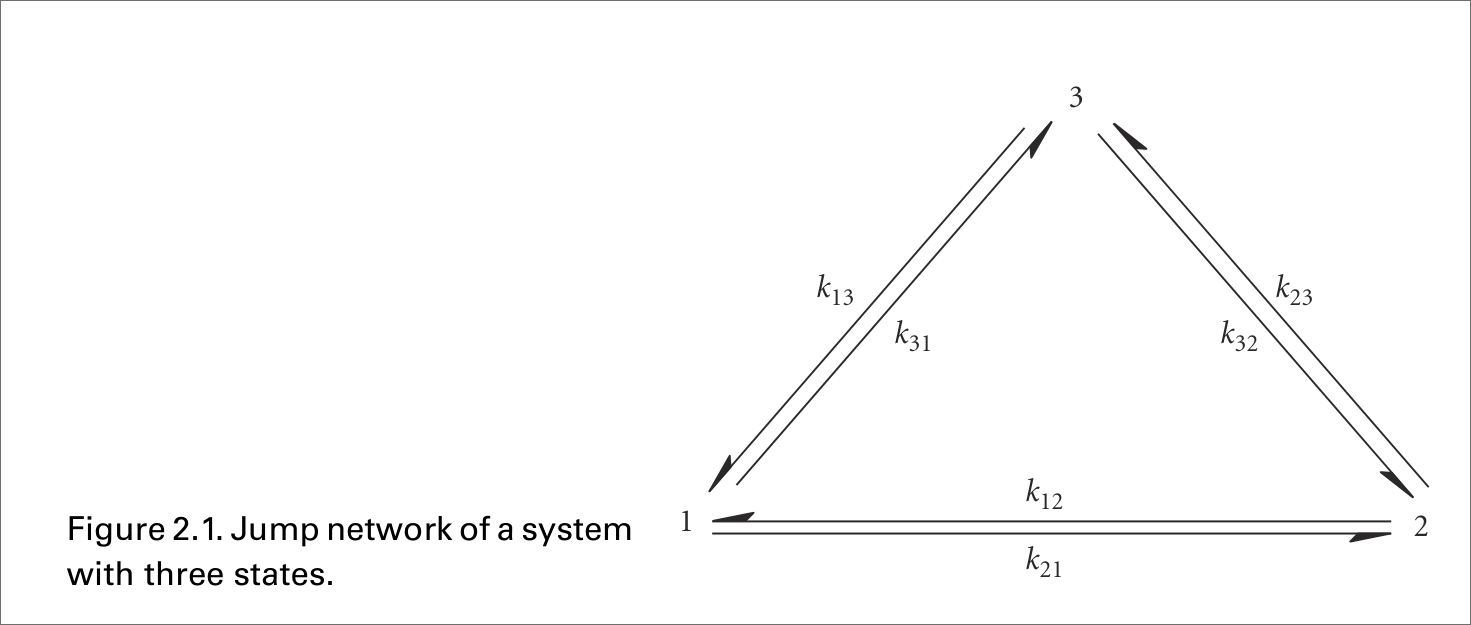
\includegraphics[width = 4in]{jump network.png}
    \caption{Source : \cite{PelitiPigolotti2023}}
  \end{figure}
\end{frame}
\section{Steady State \& Equilibrium Distribution}

\begin{frame}
  \frametitle{Conditions}
  Steady state and equilibrium distribution are often used interchangeably. However, they are defined quite differently.
  The condition for a system to be in equilibrium is a bit more constrained than that of a steady state.
  
  The necessary condition for both to hold is that the probability of being in a state $x$ at time $t$ is independent of time.
  Thus, essentially our master equation equates to $0$.
  $$\dv{p^{st}(x)}{t} = \sum_{x' \neq x} J_{xx'} = 0$$

  We will show that under certain conditions, the system relaxes to a stationary state.
  $$\lim_{t \to \infty} p(x;t) = p^{st}(x)$$
\end{frame}

\begin{frame}
  \frametitle{Detailed Balance Condition}
  The independence of $p(x)$ on time can be ensured by the following conditions:
  \begin{enumerate}
    \item $\sum_{x' \neq x} J_{xx'} = 0$
    \item $J_{xx'} = 0$ for all states $x,x'$ 
  \end{enumerate}
  Condition 1 is the condition for a steady state, while condition 2 is the condition for equilibrium.
  \begin{block}{Detailed Balance Condition}
    The detailed balance condition is defined as 
    $$k_{xx'}p^{st}(x') = k_{x'x}p^{st}(x) \quad  \forall ~x,x' \in S$$
    $$ J_{xx'}  =0 \quad \forall x,x' \in S$$
  \end{block}

    When the jump networks satisfy the detailed balance condition, the system is said to be in equilibrium.
\end{frame}

\section{Perron Frobenius Theorem}

\begin{frame}
  \frametitle{Irreducibility}
  \begin{block}{Reducibility}
    A matrix $\A$ is said to be reducible when there exists a Permutation matrix $P$ such that
    $$P^TAP = \begin{pmatrix}
      \X & \Y \\
      0 & \Z
    \end{pmatrix}$$
    where $\X$ and $\Z$ are square matrices. 
  \end{block}
  We can easily see that if all the elements of $\A$ are positive, then the matrix is irreducible.
  \emph{This is a necessary condition for the Perron Frobenius theorem to hold.}

\end{frame}
\begin{frame}
  \frametitle{Irreducibility}
  We can reframe the Irreducibility problem in terms of graphs.

  \begin{block}{Irreducibility in terms of Graphs}
    \begin{itemize}
      \item The graph $G(\A)$ of a matrix $\A_{n \times n}$ is a directed graph on $n$ nodes ${N_1,...,N_n}~$ in which there is a directed edge from $N_i$ to $N_j$ if and only if $A_{ij} \neq 0$.
      \item A graph $G(\A)$ is called strongly connected if for every pair of nodes $N_i$ and $N_j$ there is a directed path from $N_i$ to $N_j$.
      \item A matrix $\A$ is irreducible iff the graph of the matrix is strongly connected.
      \end{itemize}
    \end{block}
    We have already assumed that the jump network is strongly connected.
\end{frame}

\begin{frame}
  \frametitle{Strongly Connected Graphs}
  We can also think of Irreducibility from the point of view of the markov chains.
  Two states are said to be \textbf{communicating} if there is a non-zero probability of transitioning from one state to the other in a finite number of steps.
  This is an equivalence relation and thus partitions the state space into equivalence classes. \\ 

  The markov chain is said to be irreducible if there is only one equivalence class, which is the state space of the Markov chain.

  Here in our jump networks any state can be reached from any other state in a finite number of steps. Thus our markov chain is irreducible.

\end{frame}
\begin{frame}
  \frametitle{Strongly Connected Graphs}
  
  \begin{figure}
    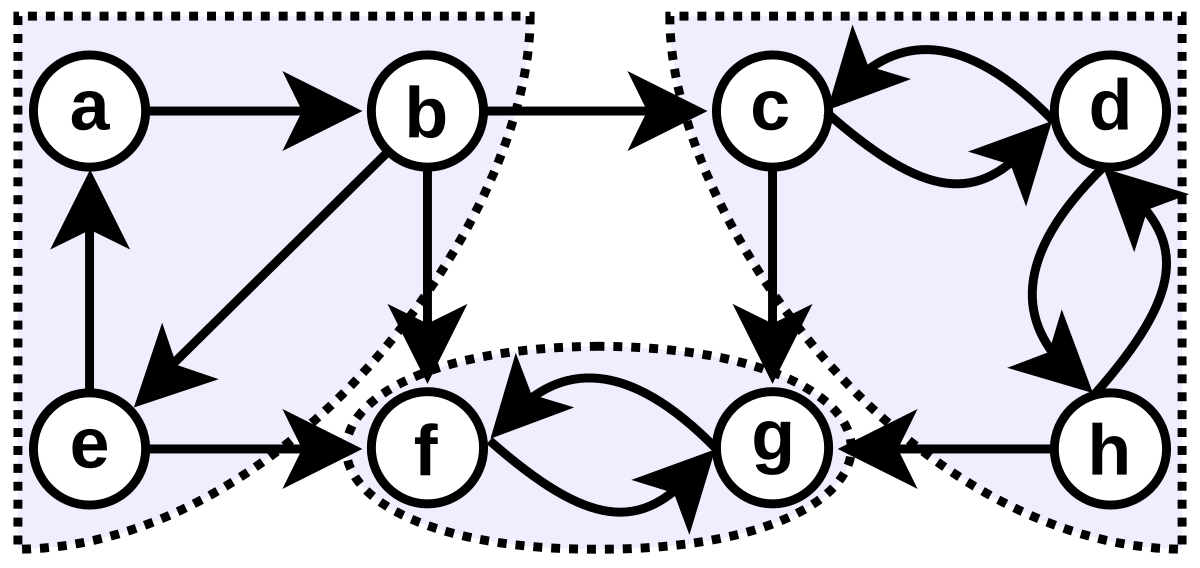
\includegraphics[width = 4in]{scc.png}
    \caption{Source : Wikipedia}
  \end{figure}
\end{frame}
\begin{frame}
  \frametitle{Primitive Matrices}
  \begin{block}{Primitive}
    \begin{itemize}
      \item A matrix $\A$ is called primitive if there exists a positive integer $k$ such that $\A^k$ is a positive matrix (i.e. all elements are positive).
      \item A matrix $\A$ is primitive if it has only one eigenvalue on the spectral circle.
      \item A non-negative irreducible matrix $\A $ is primitive with $r = \rho(\A)$ iff $\lim_{k \to \infty} (\A\slash r)^k$ exists, in which case
            $$\lim_{k \to \infty} \left(\frac{\A}{r}\right)^k = \frac{p q^{T}}{q^{T} p} > 0$$
            where $p$ and $q$ are the Perron vectors for $\A$ and $\A^T$ respectively. 
    \end{itemize}

  \end{block}
\end{frame}


\begin{frame}
  \frametitle{The Perron Frobenius Theorem}
  \begin{block}{Perron Frobenius Theorem}
    Let $\A$ be an irreducible matrix.
    \begin{itemize}
    \item There exists a positive real number $\lambda$ such that
      $$\A \pi = \lambda \pi$$ called the Perron-Frobenius eigenvalue. Moreover, the eigenvalue is the
      spectral radius of the matrix.
    \item The eigenspace corresponding to the Perron-Frobenius eigenvalue is one-dimensional, that is, the corresponding eigenvector is non-degenerate.
    \item  Then there exists a unique probability vector $\pi$ such that
    $$ \A \pi =  \lambda \pi$$ called the Perron vector. 
    Moreover, the vector $\pi$ is strictly positive.
      \item Furthermore, there are no non-negative eigenvectors of $\A$ except for all positive multiples
            of $\pi$.
    \end{itemize}
  \end{block}
\end{frame}

\begin{frame}
  \frametitle{Stationary State Distribution}
  \begin{block}{Stationary State Dist.}
  Let $P$ be the transition probability matrix for an irreducible Markov chain and 
  let $\pi$ be the perron vector for the matrix $P$. 
  \begin{itemize}
    \item The kth step probability matrix is given by
       $P^k$ since the $(i,j)$th entry of $P^k$ is the probability of transitioning from state $j$ to state $i$ in exactly $k$ steps.
    \item The $k$the step distribution is given by
      $p(k) = P^k p(0)$
      \item If $\PP$ is primitive and if $e$ denotes the column of all ones, then the limit
        $$\lim_{k \to \infty} \PP^k = \pi e^T \quad \quad \quad \text{and} \quad \quad
           \lim_{k \to \infty} p(k) = \pi$$ 

  \end{itemize}
  \end{block}


\end{frame}
\begin{frame}
  \frametitle{Stationary State Distribution}
  \underline{\textbf{Proof: }} \\ 
  All stochastic matrices $\PP$ have a spectral radius $\rho(\PP) =1$. All column sums equal to 
  1. Thus, $e$ is an eigenvector of $\PP^T$ with eigenvalue $1$, where $e$ is the column vector with 
  all ones in its entries. We also have $\norm{\PP}_{1} = 1$. Using the fact that $\rho(\star) \leq \norm{\star}$ for every matrix norm(See \cite{Meyer2000}),
  we get  that 
  $$ 1 \leq \rho(\PP) \leq \norm{\PP}_{1} = 1 ~~~ \Rightarrow \rho (\PP) =1$$

  We know that $\PP$ is primitive with $\rho(\PP) = 1$, we know that 
  $$ \lim_{k \to \infty} \PP^k = \frac{p q^T}{q^T p}  $$
  where $p$ and $q$ are the perron vectors for $\PP$ and $\PP^T$ respectively.
  The perron vector for $\PP^T$ is $e$ and let the perron vector for $\PP$ be $\pi$. 
  

\end{frame}
\begin{frame}
  \frametitle{Stationary State Distribution}

  We thus have,
  $$ \lim_{k \to \infty} \PP^k = \frac{\pi e^T}{e^T \pi}  $$
  From the conservation of probability we have that $\sum_i \pi_i =1$, we have that 
  $e^T\pi = \sum_i \pi_i = 1$.Thus we have 
  $$\lim_{k \to \infty} \PP^k = \pi e^T$$
  Now we have
  $$ \lim_{k \to \infty} p(k) = (\lim_{k \to \infty} \PP^k) p(0)= \pi e^Tp(0)$$
  Again $e^Tp(0) = \sum_i p_i(0) = 1$. This leads to 
  $$  \lim_{k \to \infty} p(k) = \pi $$

  Note that the stationary limit is independent of the initial distribution $p(0)$ here.

\end{frame}
\begin{frame}
  \frametitle{Stationary State Distribution}
  We now actually verify that $\pi$ is indeed the stationary distribution. 
  Let us recast the master equation into matrix form.
  $$ \frac{d p(t)}{dt} = Q p(t) = \frac{1}{dt}(\PP - \mathbb{I}) p(t)$$ where
  $Q$ is the transition rate matrix. Now we have 
  $$ (\PP - \mathbb{I})\pi = \PP \pi - \pi = \pi -\pi = 0 $$
  Thus the infinite time limit of the probability distribution is indeed the stationary distribution.
  $$  \Rightarrow  \frac{d \pi }{dt} = 0$$

  Now the stationary distribution must be unique since the Perron root of any irreducible 
  matrix has a one dimensional eigenspace. Thus the eigenvector must be unique due to 
  the conservation of probability.
  \hfill \square
\end{frame}

\begin{frame}
  \frametitle{Stationary state Distribution}
  SIDE NOTE: After completing the presentation, I found a proof that doesn't use Perron Frobenius theorem. However, that only proves it 
  for a transition rate matrix with all positive entries.\cite{PelitiPigolotti2023}
\end{frame}
\begin{frame}
  \frametitle{Stationary state Distribution}
  \begin{block}{Stationary State Dist. for Imprimitive matrices}
  Let $P$ be the transition probability matrix for an irreducible Markov chain and 
  let $\pi$ be the perron vector for the matrix $P$. 
  \begin{itemize}
      \item If $\PP$ is imprimitive and if $e$ denotes the column of all ones, then the limit
        $$\lim_{k \to \infty} \frac{\mathbb{I} + \PP + ... +\PP^{k-1}}{k} = \pi e^T $$ and 
        
        $$ \lim_{k \to \infty} \frac{p(0) + p(1) + ...+p(k-1)}{k} = \pi$$ 
  \end{itemize}
  \end{block}

  We use Cesaro sums to define the stationary state probability distribution. However, we won't deal with it here. 

\end{frame}
\section{Graph Theory}
\begin{frame}
  \frametitle{Preliminaries}
  \begin{itemize}
   \item A graph is a collection of vertices and edges. The edges connect the vertices.
   \item The degree of a vertex is the number of edges connected to it.
   \item A walk is a sequence of vertices connected by edges.
   \item A trail is a walk with no repeated edges.
   \item A cycle is a non-empty trail that starts and ends at the same vertex.
   \item A connected graph is a graph where there is a path between every pair of vertices.
  \end{itemize}

\end{frame}
\begin{frame}
  \frametitle{Trees}
  \begin{block}{Trees}
    A tree is a connected graph with no cycles.
  \end{block}
  Here is one property of a tree that we plan to use later.
  \\ 
   A tree with $n$ vertices has $n-1$ edges.
\end{frame}
\begin{frame}
  \frametitle{Handshaking Lemma}
  \begin{block}{Handshaking Lemma}
    The sum of the degrees of all the vertices of a graph is equal to twice the number of edges. \\
    $$\sum_{i=1}^{n} d_i = 2|E|$$
    where $d_i$ is the degree of the $i$th vertex and $|E|$ is the number of edges.
    \end{block}    

\end{frame}
\begin{frame}
  \frametitle{An "obvious" Theorem}
  \begin{block}{An "obvious" Theorem}
    A tree has at least two vertices of degree 1.

  \end{block}
  \underline{\textbf{Proof}}\\
  Every tree has $n-1$ edges, so  the sum of the degrees of all vertices of any tree 
  has to be $2(n-1)$. But if there are fewer than two vertices of degree one, 
  then the sum of the degrees of all vertices must be at least $2(n-1)+1$, 
  which is a contradiction.

  \hfill \square




\end{frame}
\section{Equilibrium Distribution}
\begin{frame}
    \frametitle{Trees}
    \begin{block}{Equilibrium dist. for trees}
      Let the jump network be a tree. Then the stationary state distribution is the equilibrium distribution.
      \end{block}
      \underline{\textbf{Proof}}\\
      We know that there exists at least $2$ vertices with degree $1$. Let us label one of them as $x$.
      Thus, for this vertex $\sum_{x' \neq x} J_{xx'} = 0$ for all states $x'$ connected to it, under the stationary distribution.
      Since this is only connected to another vertex say $a$, We have $J_{xa} = 0$. We can then remove the vertex $x$ and the edge $\{x,a\}$.
      This is still a tree, so we can do this iteratively. We can reach a point where we have only one vertex left. For the lone vertex,
      the detailed balance condition is trivially satisfied. Thus, the equilibrium distribution is the stationary distribution.

      \hfill \square

    
  
\end{frame}
\begin{frame}
  \frametitle{Cyclic Networks}
  \begin{block}{Cyclic Network}
    A cyclic network is a graph with a cycle in it.
  \end{block}
  \begin{block}{Cyclic Networks}
    For cyclic networks, the system admits an equilibrium distribution if 
    for any sequence states $(x_0,...,x_n)$ all different from each other
    $$k_{x_0x_1}k_{x_1x_2}...k_{x_{n-1}x_n}k_{x_nx_0} = k_{x_0x_n}k_{x_nx_{n-1}}...k_{x_1x_0}$$
    \end{block}
    We can see that non-vanishing stationary currents can only survive in loops. If we allow for all cycles the forward and back jump rates to be equal, we can then allow for 
    the balance of probability currents.

\end{frame}

\begin{frame}
  \frametitle{Note}
  \begin{block}{Admission of Equilibrium Distribution}
    For cyclic networks, the system admits an equilibrium distribution if 
    for any sequence states $(x_0,...,x_n)$ all different from each other
    $$k_{x_0x_1}k_{x_1x_2}...k_{x_{n-1}x_n}k_{x_nx_0} = k_{x_0x_n}k_{x_nx_{n-1}}...k_{x_1x_0}$$
    \end{block}
    Note that this also includes the acyclic cases as well. For all sequences $(x_0,...,x_n)$ that is not a cycle with $x_0$
    we  get $k_{x_0 x_n} = k_{x_n x_0} = 0$. Thus, this condition is trivially satisfied for acyclic networks.
\end{frame}

\begin{frame}[standout]

  Questions?
\end{frame}
\section{Danke Schön}
\begin{frame}
  \frametitle{References}
  \begin{thebibliography}{99}

    \bibitem{PelitiPigolotti2023}
    Luca Peliti and Simone Pigolotti, \textit{Stochastic Thermodynamics}, 
    Princeton University Press, Princeton, NJ, 2023.
    
    \bibitem{Meyer2000}
    Carl D. Meyer, \textit{Applied Linear Algebra and Matrix Analysis}, 
    Society for Industrial and Applied Mathematics (SIAM), Philadelphia, PA, 2000.
    
    \end{thebibliography}

\end{frame}
\end{document}